\documentclass[12pt]{beamer}
\usepackage[utf8]{inputenc}
\usepackage[T1]{fontenc}
\usepackage{lmodern}
%\usetheme{Malmoe}
%\usetheme{Warsaw}
\usepackage{graphicx}
\usepackage{newverbs}

\newverbcommand{\tc}{\color{blue}}{}

%\usebackgroundtemplate{\includegraphics[width=\paperwidth,height=\paperheight]{./images/background.jpg}}

\begin{document}
	\author{Fedora QA}
	\title{Two heads are better than one}
	\subtitle{or How to use Fedora Test Days to test for you}
	\titlegraphic{
\includegraphics[width=3cm]{logo.png}}
	\institute{Lukáš Růžicka (lruzicka@redhat.com)}
	\date{}
%	\subject{Fedora 29}
	%\setbeamercovered{transparent}
	%\setbeamertemplate{navigation symbols}{}

\begin{frame}[plain]
	\maketitle
\end{frame}



%{\usebackgroundtemplate{
\includegraphics[width=\paperwidth]{./images/alone.png}}
\begin{frame}
\frametitle{When you test alone}
\begin{center}
	
\includegraphics[width=10cm]{images/alone.png}
\end{center}
\end{frame}

{%\usebackgroundtemplate{\includegraphics[width=\paperwidth]{./images/crowd.png}}
\begin{frame}
\frametitle{When community helps you}
	% When community helps testing:
	% - they might not know the functionality
	% - they test for they think (and want) to achieve with it
	% - they test with different approach
	% - they test with different hardware
	% - they can be numerous and produce more results
	% Result: Various problems can be caught.
	\begin{center}
		
\includegraphics[width=10cm]{images/community.png}
	\end{center}
\end{frame}}


\begin{frame}
\frametitle{Fedora Test Days}
	\begin{center}
	
\includegraphics[width=10cm]{images/testdays.png}
	\end{center}
%Test days are events organized by Fedora QE to get the community involved in testing. \linebreak
%The Fedora Days
%
%\begin{itemize}
%	\item focus on a particular part of the release (apps, features, enhancements, bug fixing),
%	\item take place between \textbf{Alpha} (branching out) and \textbf{GA} milestones,
%	\item provide guidelines to community testers,
%	\item provide online assistance from Fedora QE staff,
%	\item and collect test results.
%\end{itemize}
\end{frame}

\begin{frame}
\frametitle{Previously organized Test Days (Fedora 29)}
	\begin{center}
	
\includegraphics[width=10cm]{images/previous.png}
	\end{center}
%\begin{itemize}
%	\item Kernel (4.17, 4.18, 4.19)
%	\item Fedora Media Writer
%	\item DNF 3.5.1
%	\item Gnome 3.30
%	\item Silverblue
%	\item Modularity
%	\item more at {\color{blue}\url{http://testdays.fedorainfracloud.org/events}}
%\end{itemize}

\end{frame}

\begin{frame}
\frametitle{How to run your own Test Day?}
%Follow {\color{blue}\url{https://fedoraproject.org/wiki/QA/SOP_Test_Day_management}}. 
\begin{center}
	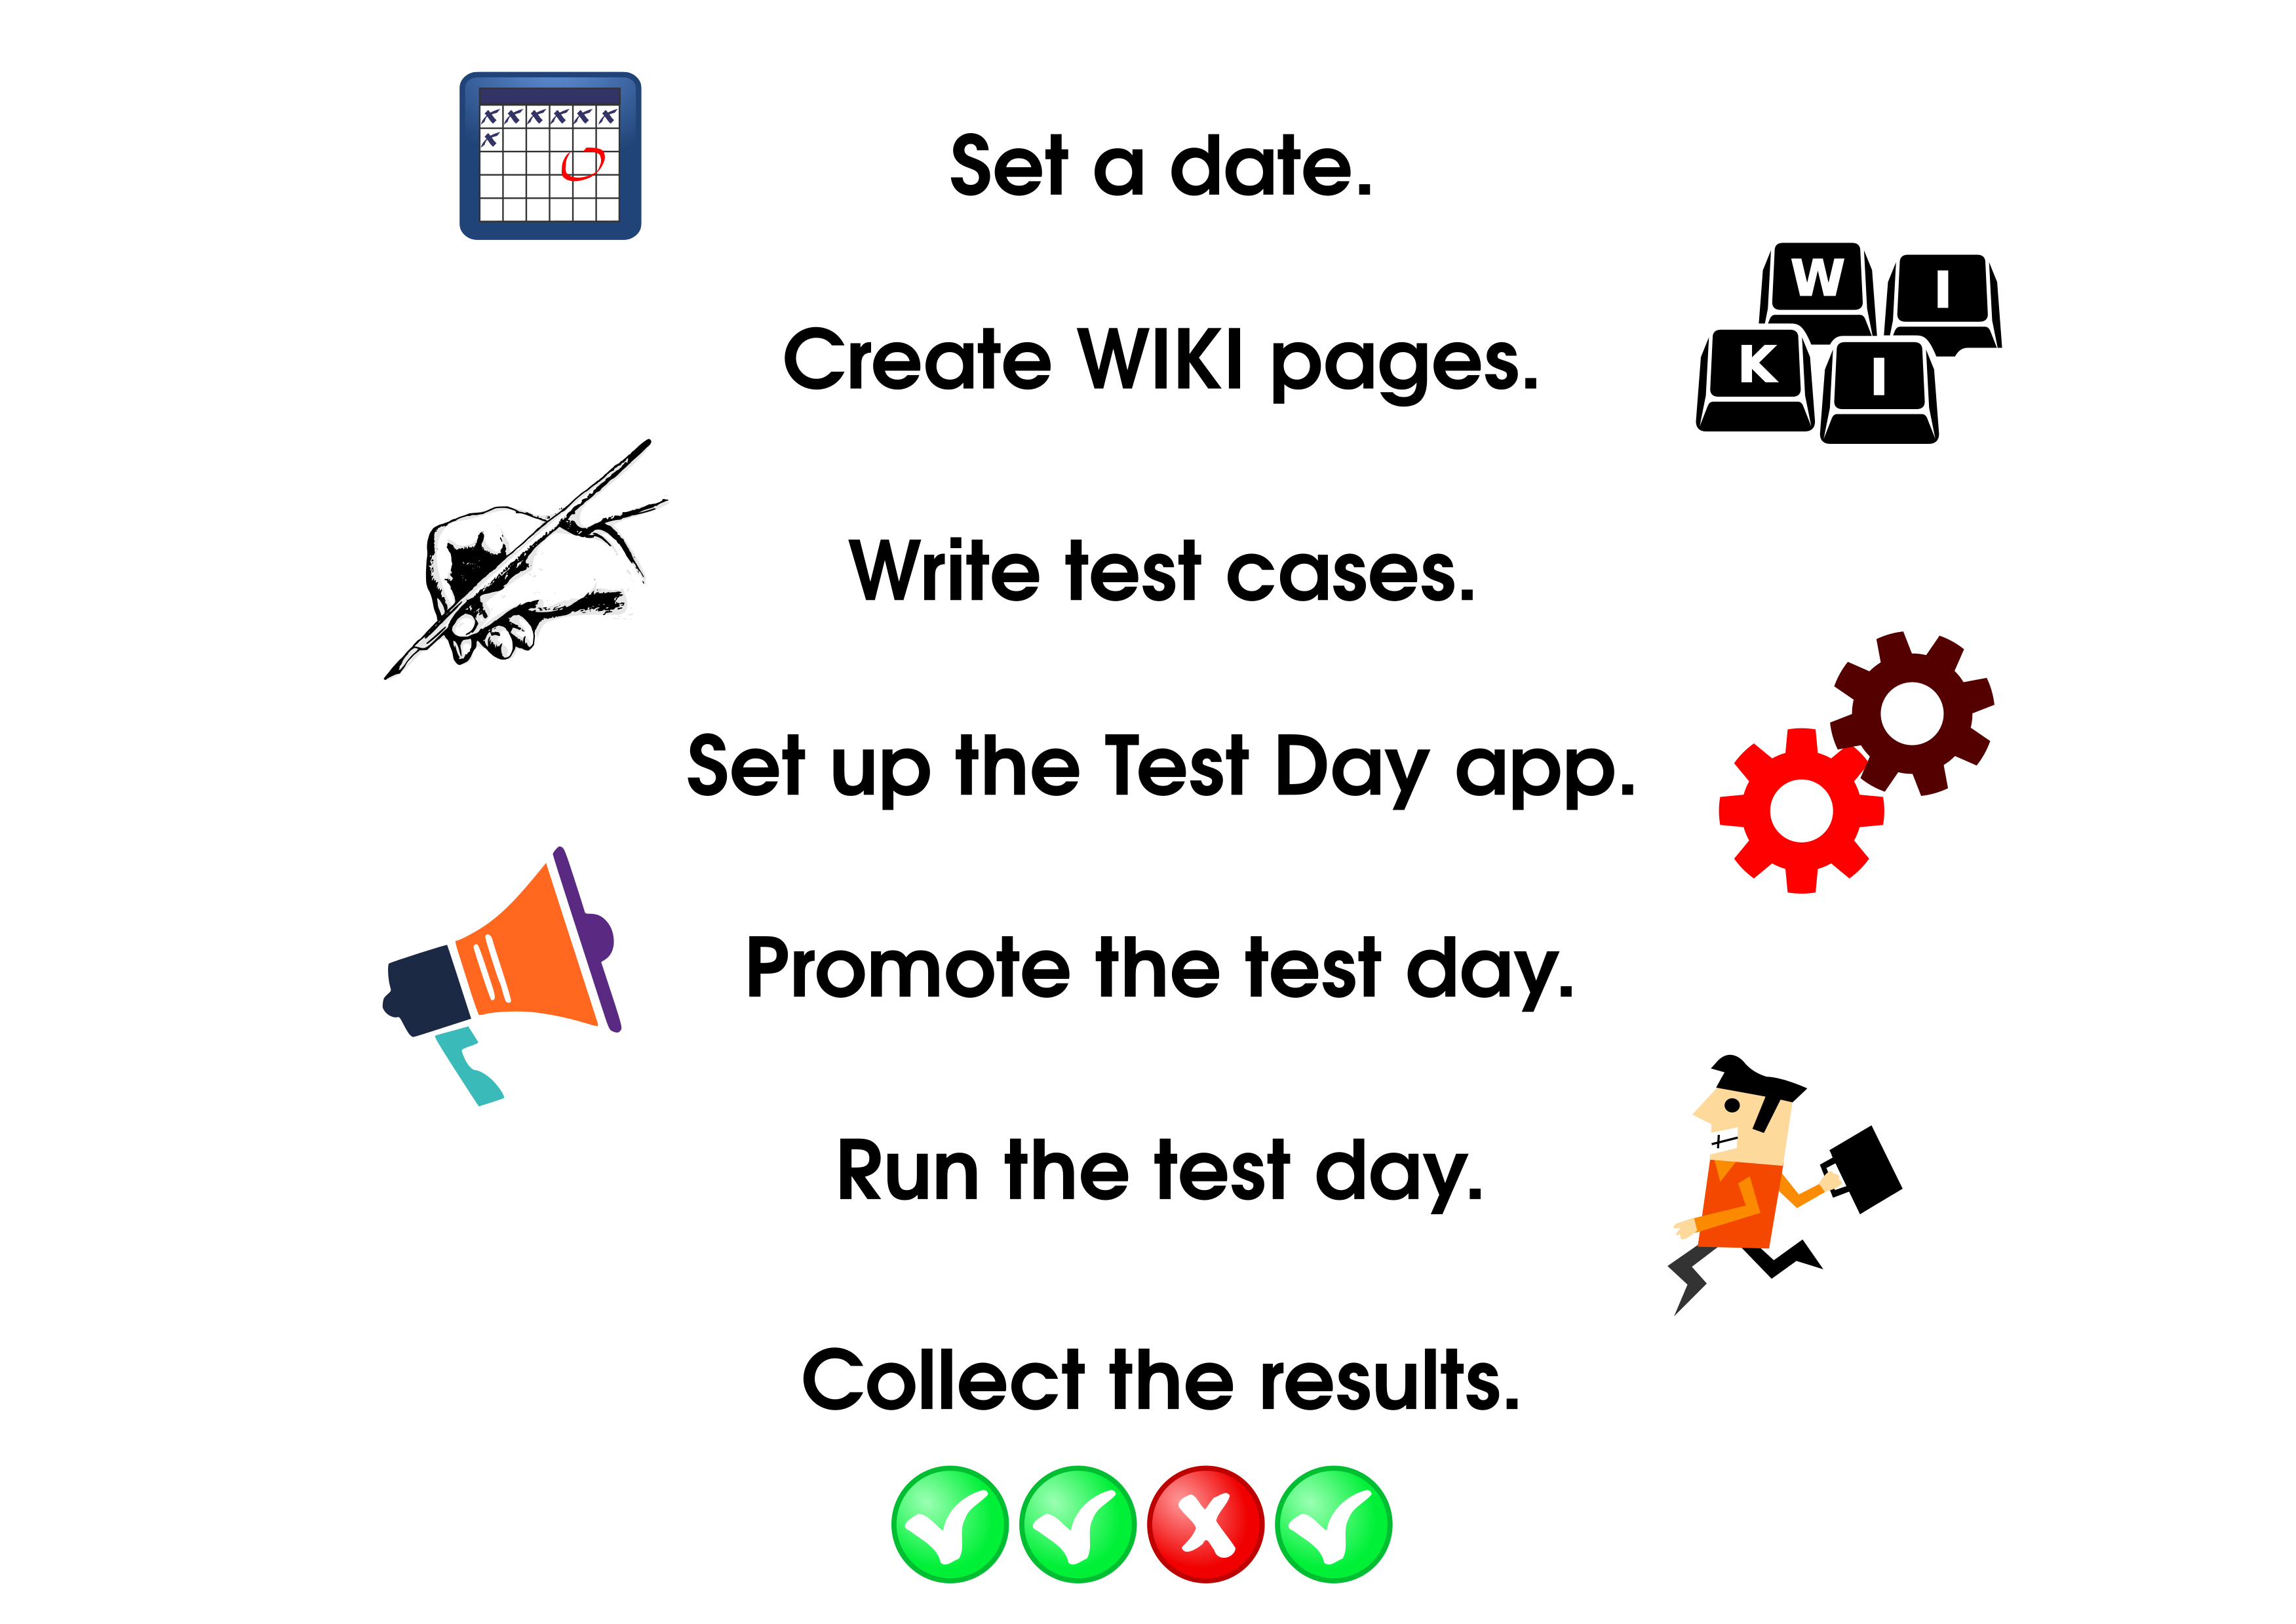
\includegraphics[width=10cm]{images/howtorun.png}
\end{center}

%\begin{itemize}
%		\item set a date,
%		\item create necessary Wiki pages,
%		\item write test cases,
%		\item set up the Test Day App,
%		\item promote the Test Day,
%		\item run it,
%		\item and collect results.
%\end{itemize}
\end{frame}

\begin{frame}
\frametitle{Too busy to do it?}
\begin{center}
	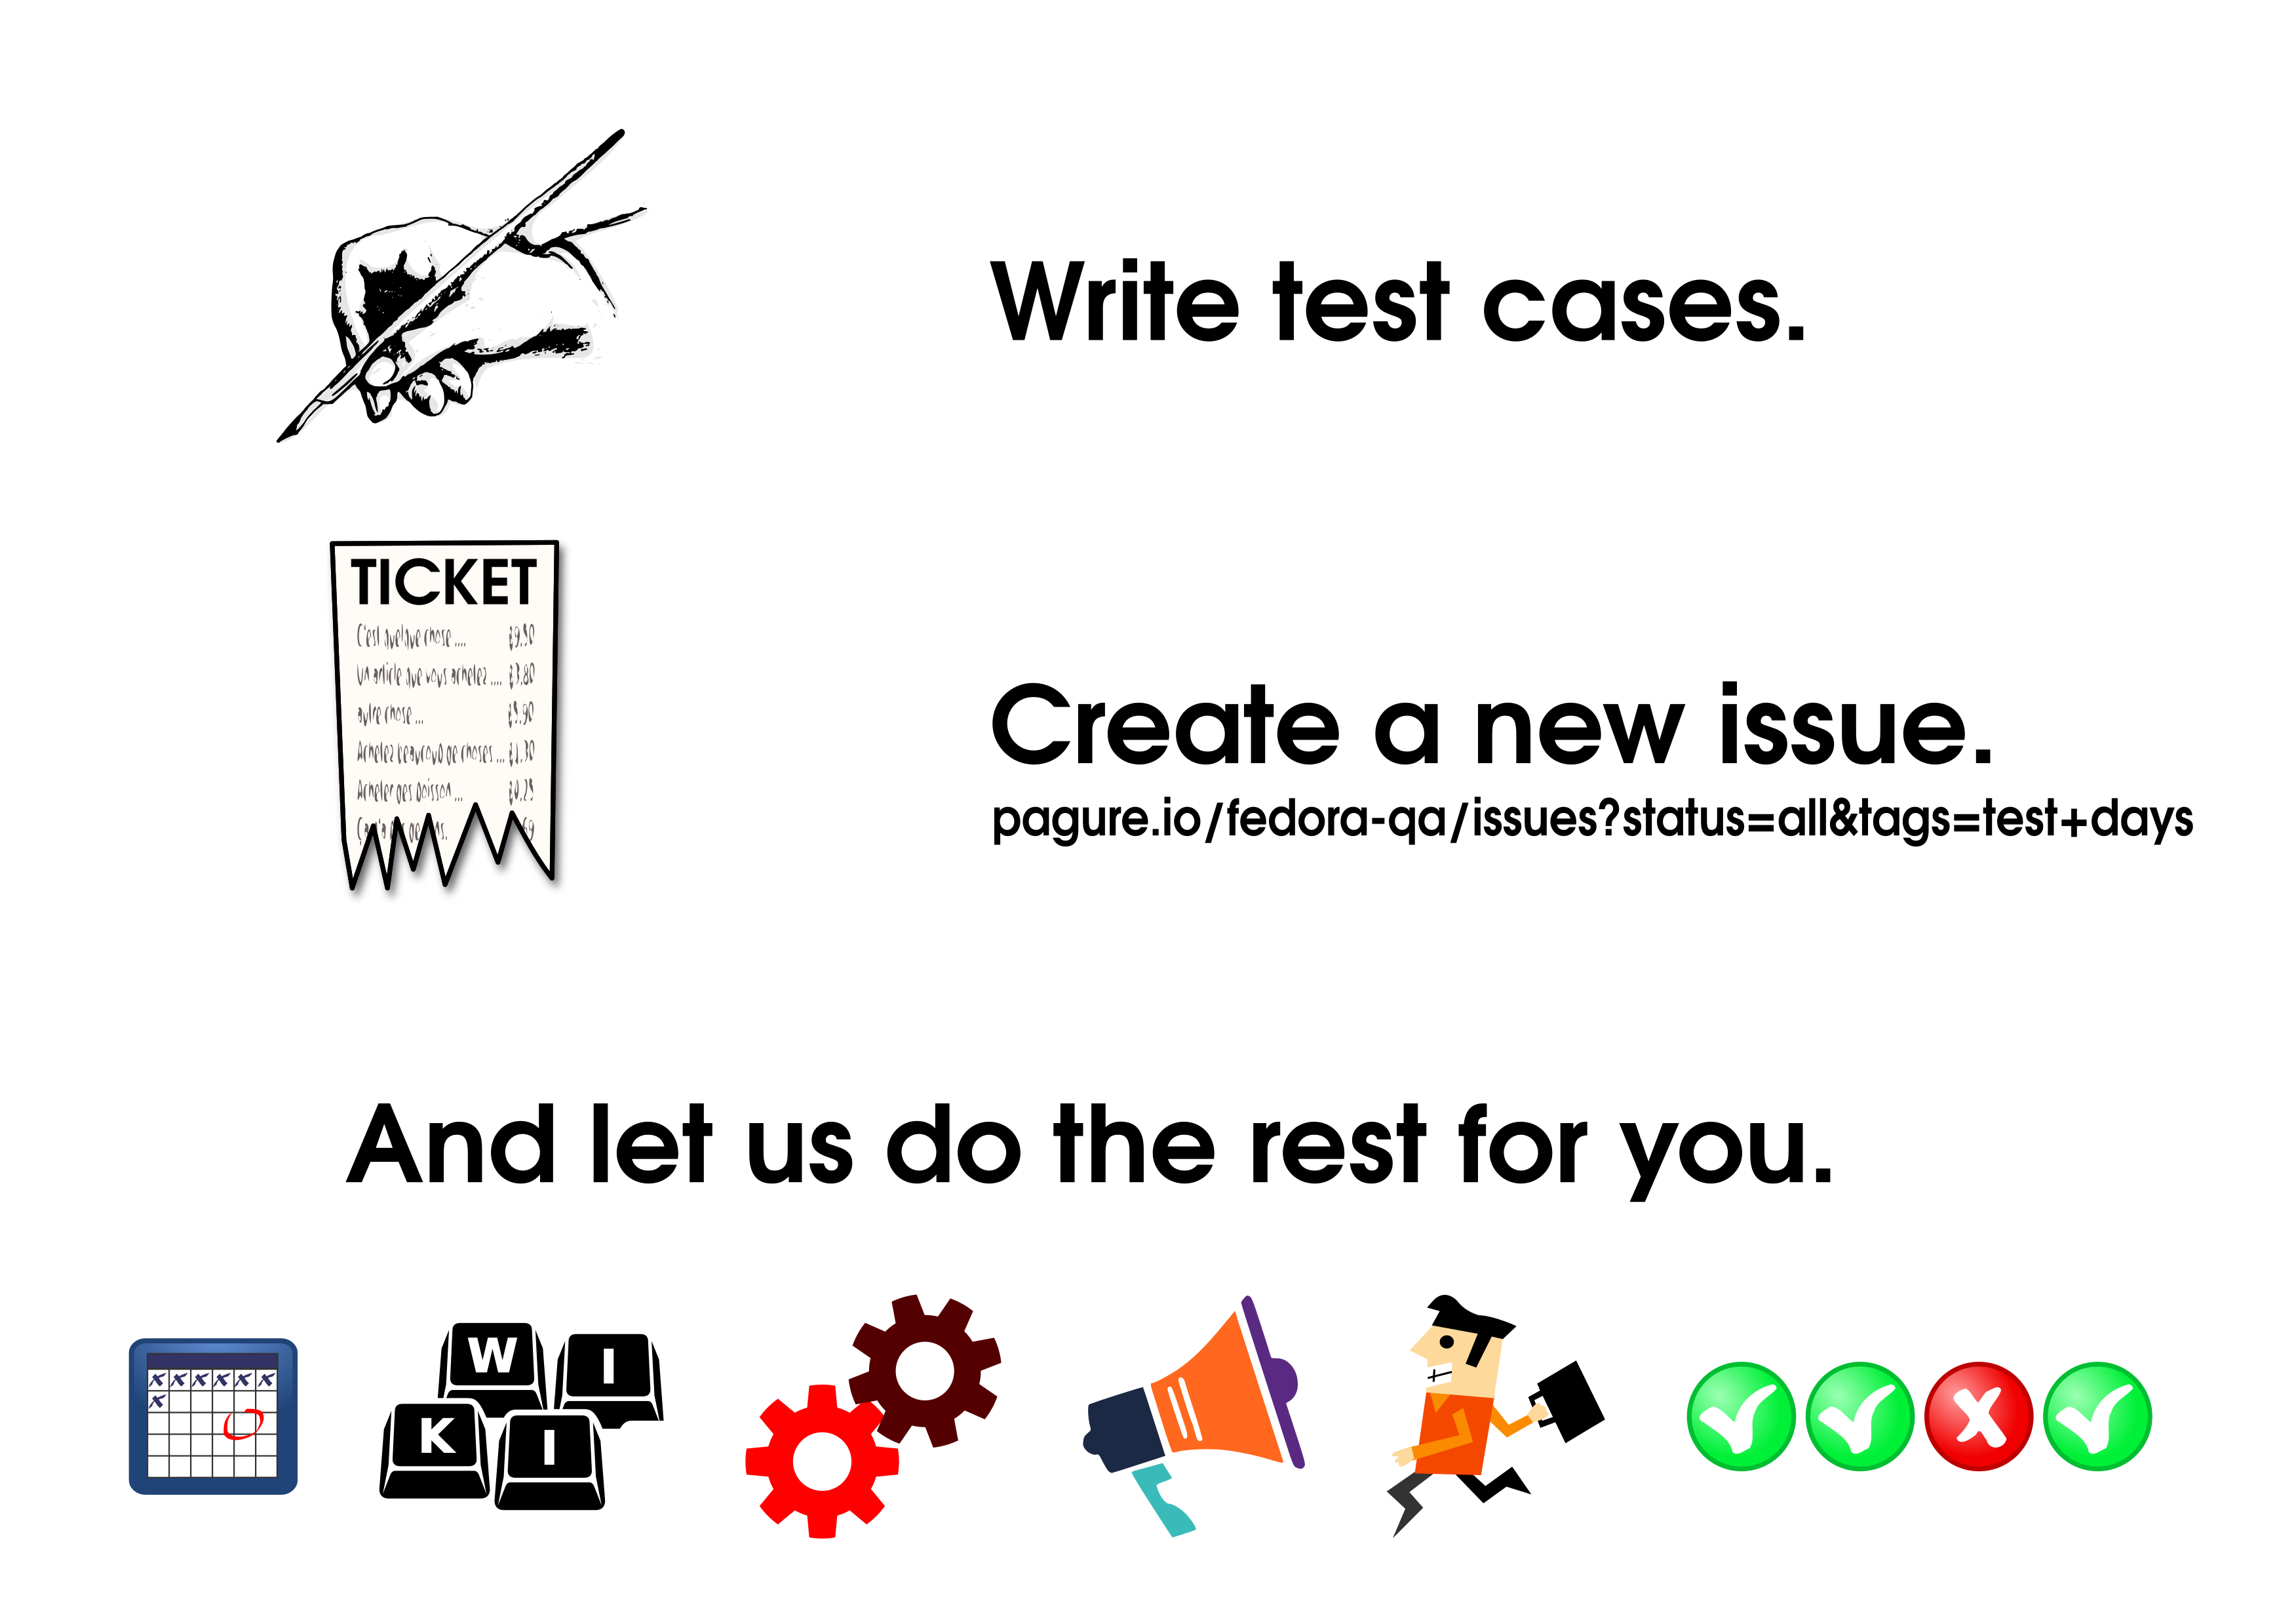
\includegraphics[width=10cm]{images/toobusy.png}
\end{center}
%\begin{itemize}
%	\item Create an issue to propose the Test Day at {\color{blue}\url{https://pagure.io/fedora-qa/issues?status=all&tags=test+days}},
%	\item give us some details,
%	\item prepare the test cases,
%	\item let us help you run the event,
%	\item or let us run it for you.
%\end{itemize}

\end{frame}

\begin{frame}
\frametitle{Interested?}

Points of contact:

\begin{itemize}
	\item Sumantro Mukherjee, sumantro, (sumukher@redhat.com)
	\item František Zatloukal, frantisekz, (fzatlouk@redhat.com)
	\item Kamil Páral, kparal, (kparal@redhat.com)
	\item Lukáš Brabec, lbrabec, (lbrabec@redhat.com)
	\item Lukáš Růžička, lruzicka, (lruzicka@redhat.com)
	\item \#fedora-qa @ freenode
\end{itemize}

\end{frame}

\end{document}